\documentclass[aspectratio=169,11pt]{beamer}

\usepackage[T1]{fontenc}
\usepackage{lmodern}
\usepackage{tikz}
\usepackage[most]{tcolorbox}

% ---------- colors ----------
\definecolor{deep}{HTML}{14424F}
\definecolor{teal}{HTML}{1F6F7A}
\definecolor{amber}{HTML}{F2A541}
\definecolor{tint}{HTML}{E9F1F3}
\definecolor{ink}{HTML}{1A2B33}
\definecolor{muted}{HTML}{6B7C88}

\setbeamercolor{normal text}{fg=ink,bg=white}
\setbeamercolor{frametitle}{fg=deep,bg=white}
\setbeamercolor{framesubtitle}{fg=muted}
\setbeamercolor{itemize item}{fg=teal}
\setbeamercolor{itemize subitem}{fg=teal}
\setbeamercolor{alerted text}{fg=teal}
\setbeamerfont{frametitle}{size=\LARGE,series=\bfseries}
\setbeamerfont{framesubtitle}{size=\footnotesize,shape=\itshape}
\setbeamertemplate{navigation symbols}{}
\setbeamertemplate{itemize item}[circle]
\setbeamertemplate{itemize subitem}[circle]
\setbeamertemplate{footline}{%
  \hspace{1.2em}{\color{muted}\scriptsize CSL559 Computer System Design \;|\; Paper Discussion 2}%
  \hfill{\color{muted}\scriptsize\insertframenumber}\hspace{1.2em}\vspace{0.6em}}
\setlength{\leftmargini}{1.1em}

% ---------- helpers ----------
\newcommand{\num}[1]{\tikz[baseline=(c.base)]\node[circle,fill=amber,text=deep,inner sep=1.5pt,minimum size=1.5em,font=\bfseries\large](c){#1};}

\newtcolorbox{infobox}[1]{enhanced,colback=tint,colframe=tint,arc=2mm,
  left=2mm,right=2mm,top=1.2mm,bottom=1.2mm,boxsep=0pt,
  fontupper=\small\raggedright,before upper={{\color{teal}\scriptsize\bfseries #1}\par\smallskip}}

\newcommand{\term}[2]{{\color{deep}\bfseries #1:} #2\par\vspace{1.5pt}}
\newcommand{\head}[1]{{\color{teal}\scriptsize\bfseries #1}\par\smallskip}

\newcommand{\vstat}[2]{%
  \begin{tcolorbox}[enhanced,colback=deep,colframe=deep,arc=2mm,left=2.5mm,right=1mm,top=1.6mm,bottom=1.4mm,boxsep=0pt,before skip=0pt,after skip=1.2mm]
    \raggedright{\color{amber}\normalsize\bfseries #1}\par{\color{white}\scriptsize #2}
  \end{tcolorbox}}

% Part 1 of a paper: #1 number, #2 name, #3 full title + venue, #4 problem items, #5 idea, #6 key terms
\newcommand{\partA}[6]{%
\begin{frame}
  \frametitle{\num{#1}\; #2}
  \framesubtitle{#3}
  \vspace*{-3mm}
  \begin{columns}[T,onlytextwidth]
    \begin{column}{0.49\textwidth}
      \begin{infobox}{THE PROBLEM}\normalsize
        \begin{itemize}\setlength{\itemsep}{5pt}
          #4
        \end{itemize}
      \end{infobox}
    \end{column}
    \begin{column}{0.48\textwidth}
      \begin{infobox}{MAIN IDEA}\normalsize #5\end{infobox}
      \vspace{1.5mm}
      \begin{infobox}{KEY TERMS}#6\end{infobox}
    \end{column}
  \end{columns}
\end{frame}}

% Part 2 of a paper: #1 number, #2 short name, #3 how items, #4 stats, #5 takeaway
\newcommand{\partB}[5]{%
\begin{frame}
  \frametitle{\num{#1}\; #2: how it works}
  \vspace*{-2mm}
  \begin{columns}[T,onlytextwidth]
    \begin{column}{0.61\textwidth}
      \head{HOW IT WORKS}
      \small
      \begin{itemize}\setlength{\itemsep}{3pt}
        #3
      \end{itemize}
    \end{column}
    \begin{column}{0.36\textwidth}
      \head{RESULTS}
      #4
    \end{column}
  \end{columns}
  \vspace{1mm}
  \begin{infobox}{KEY TAKEAWAY}\normalsize #5\end{infobox}
\end{frame}}

\title{From Bigtable to the Lakehouse}
\author{Paritosh Lahre}

\begin{document}

% ---------- title ----------
{
\setbeamercolor{background canvas}{bg=deep}
\setbeamertemplate{footline}{}
\begin{frame}[plain]
  \vspace{1.2cm}
  {\color{white}\fontsize{30}{34}\selectfont\bfseries From Bigtable to the Lakehouse\par}
  \vspace{4mm}
  {\color{amber}\large Paper Discussion 2: a summary of 7 papers on large-scale data systems\par}
  \vspace{1cm}
  {\color{white}\large\bfseries Paritosh Lahre\par}
  {\color{white} ID: 12341550\par}
  {\color{white} CSL559 -- Computer System Design\par}
\end{frame}
}

% ---------- big picture ----------
\begin{frame}
  \frametitle{The big picture}
  \framesubtitle{How large-scale data systems changed from 2006 to 2024}
  \centering
  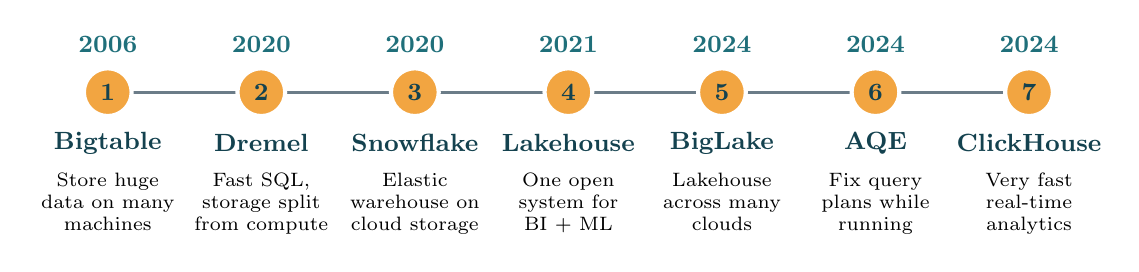
\begin{tikzpicture}[x=1.95cm]
    \draw[muted,line width=1pt] (0,0) -- (6,0);
    \foreach \i/\yr/\name/\what in {
      0/2006/Bigtable/{Store huge data on many machines},
      1/2020/Dremel/{Fast SQL, storage split from compute},
      2/2020/Snowflake/{Elastic warehouse on cloud storage},
      3/2021/Lakehouse/{One open system for BI + ML},
      4/2024/BigLake/{Lakehouse across many clouds},
      5/2024/AQE/{Fix query plans while running},
      6/2024/ClickHouse/{Very fast real-time analytics}} {
      \node[font=\bfseries\small,text=teal] at (\i,0.6) {\yr};
      \node[circle,fill=amber,draw=white,line width=1.5pt,minimum size=0.6cm,font=\bfseries\small,text=deep] at (\i,0) {\the\numexpr\i+1\relax};
      \node[font=\bfseries\small,text=deep] at (\i,-0.65) {\name};
      \node[font=\scriptsize,text width=1.8cm,align=center,anchor=north] at (\i,-0.9) {\what};
    }
  \end{tikzpicture}
  \vspace{4mm}
  \begin{infobox}{THE STORY}
    First store big data, then query it fast, then split storage from compute, then put everything on open files in the cloud.
  \end{infobox}
\end{frame}

% ================= 1. BIGTABLE =================
\partA{1}{Bigtable}
  {Bigtable: A Distributed Storage System for Structured Data \;(OSDI 2006, Google)}
  {\item Google had petabytes of data: web pages, Google Earth images, Analytics data
   \item Normal databases could not spread this over thousands of cheap machines
   \item Apps had very different needs: big batch jobs vs.\ very fast single reads}
  {A huge, sparse, sorted map. Each value is found by \alert{(row key, column key, timestamp)}. No full SQL: the app decides how to lay out its data.}
  {\term{Tablet}{a range of rows; the unit of load balancing}
   \term{Memtable}{recent writes kept in memory}
   \term{SSTable}{a sorted, read-only file stored on GFS}}

\partB{1}{Bigtable}
  {\item Tables split by row range into tablets (100--200\,MB)
   \item Master assigns tablets to servers, balances load
   \item Files on GFS; Chubby lock service keeps one master
   \item Column families; each cell keeps many versions
   \item Writes: commit log + memtable, then SSTable
   \item Compactions merge SSTables in the background
   \item Reads: Bloom filters, caching, compression}
  {\vstat{60+}{Google products used it}
   \vstat{1000s}{of servers per cluster}
   \vstat{HBase, Cassandra}{inspired by it}}
  {A simple data model plus smart storage (log, memtable, SSTable) is enough to scale to thousands of machines.}

% ================= 2. DREMEL =================
\partA{2}{Dremel}
  {Dremel: A Decade of Interactive SQL Analysis at Web Scale \;(VLDB 2020, Google)}
  {\item Analysts wanted answers in seconds over trillions of rows
   \item MapReduce jobs took minutes or hours, too slow for exploring data
   \item Data was huge, nested, and spread over many files}
  {Run SQL on data where it already lives, using \alert{column storage} and a big \alert{shared pool} of machines.}
  {\term{In situ}{query files in place, with no loading step}
   \term{Disaggregation}{storage and compute scale on their own}
   \term{Serverless}{users never set up or manage machines}}

\partB{2}{Dremel}
  {\item Its SQL became standard SQL, shared with Spanner
   \item Data in a shared file system (GFS, then Colossus)
   \item Nested columns: repetition + definition levels
   \item Reads only the columns a query needs
   \item Serving tree: root splits query, leaves scan data
   \item In-memory shuffle for big joins and group-bys
   \item One shared pool of machines for all users}
  {\vstat{2010}{BigQuery launched on Dremel}
   \vstat{Seconds}{on trillions of rows}
   \vstat{Standard}{ideas now used industry-wide}}
  {Column storage plus a large shared pool of compute makes SQL on huge data feel interactive.}

% ================= 3. SNOWFLAKE =================
\partA{3}{Snowflake}
  {Building An Elastic Query Engine on Disaggregated Storage \;(NSDI 2020, Snowflake + Cornell)}
  {\item Old warehouses are \alert{shared-nothing}: each node owns part of the data
   \item Adding or removing nodes means moving lots of data around
   \item Mixed workloads: hardware is either wasted or too small}
  {Keep tables in cloud storage (S3). Run queries on separate \alert{virtual warehouses} that can grow or shrink at any time.}
  {\term{Virtual warehouse}{a group of VMs that runs queries}
   \term{Ephemeral storage}{temp data kept on compute nodes}
   \term{Work stealing}{an idle node takes tasks from a busy one}}

\partB{3}{Snowflake}
  {\item Layers: cloud services, compute (VMs), S3 storage
   \item Cloud services: metadata, planning, scheduling
   \item Own ephemeral storage for intermediate data
   \item It also caches table files read from S3
   \item Consistent hashing for cache, no big reshuffle
   \item Work stealing handles skewed (uneven) tasks
   \item Study: $\sim$70 million queries, 14 days (Feb 2018)}
  {\vstat{59\%}{queries both read and write}
   \vstat{60--80\%}{cache hit rate}
   \vstat{$\sim$20\%}{clusters use elastic scaling}}
  {Splitting storage from compute gives elasticity, but a fast middle layer (ephemeral storage + cache) keeps queries fast.}

% ================= 4. LAKEHOUSE =================
\partA{4}{Lakehouse}
  {Lakehouse: A New Generation of Open Platforms \;(CIDR 2021, Databricks)}
  {\item Two tiers: a \alert{data lake} (cheap open files) + a \alert{warehouse} (fast SQL)
   \item ETL copies data between them: stale data, double cost, more failures
   \item ML tools cannot easily read data inside the warehouse}
  {One system: open files (Parquet) on cheap cloud storage, plus a \alert{metadata layer} that adds warehouse features on top.}
  {\term{Data lake}{raw files in cloud object storage}
   \term{ACID}{safe, all-or-nothing updates}
   \term{Delta Lake}{a transaction log on top of Parquet files}}

\partB{4}{Lakehouse}
  {\item Metadata layer (Delta, Iceberg, Hudi) keeps a log
   \item Gives ACID, time travel and schema checks
   \item Hot data cached on fast local SSDs
   \item Min/max stats per file help skip data
   \item Z-order layout keeps related rows together
   \item DataFrame APIs let ML tools read the same tables}
  {\vstat{1 copy}{of data, not lake + warehouse}
   \vstat{Open}{formats, no vendor lock-in}
   \vstat{TPC-DS}{competitive with warehouses}}
  {Warehouse features can live on open files, so one copy of data serves both BI and ML.}

% ================= 5. BIGLAKE =================
\partA{5}{BigLake}
  {BigLake: BigQuery's Evolution toward a Multi-Cloud Lakehouse \;(SIGMOD 2024, Google)}
  {\item Data sits in open formats on Google Cloud, AWS S3 and Azure
   \item Customers want BigQuery's security and speed on this data
   \item Other engines (Spark, Presto) must use the same data safely}
  {Bring BigQuery's \alert{security rules} and \alert{fast query engine} to open-format data, in any cloud.}
  {\term{Fine-grained security}{access control per row and column}
   \term{Apache Iceberg}{an open table format}
   \term{Object table}{a table view over images or documents}}

\partB{5}{BigLake}
  {\item Row and column security on files in storage
   \item Users never need direct access to the files
   \item Read/Write APIs: Spark, Presto follow same rules
   \item Metadata caching to skip files, plan faster
   \item Managed tables use the Iceberg format
   \item Object tables: images/docs, ML from SQL
   \item BigQuery Omni runs Dremel in AWS and Azure}
  {\vstat{5$\times$}{faster Spark reads (Read API)}
   \vstat{3 clouds}{Google Cloud, AWS, Azure}
   \vstat{Cross-cloud}{joins without copying data}}
  {A lakehouse can be multi-cloud: one place for security rules and queries, wherever the data is stored.}

% ================= 6. AQE =================
\partA{6}{Adaptive Query Execution (AQE)}
  {Adaptive and Robust Query Execution for Lakehouses at Scale \;(VLDB 2024, Databricks)}
  {\item Table stats are often missing or old (raw data, fast ingestion)
   \item Size guesses for filters, joins and UDFs are often wrong
   \item A fixed plan then causes heavy data movement, disk spill and memory pressure}
  {Don't trust the first plan. When a stage finishes, use the \alert{real data sizes} to re-plan the rest of the query.}
  {\term{Shuffle}{moving data between machines by key}
   \term{Broadcast join}{send the small table to every machine}
   \term{Skew}{one partition much bigger than the rest}}

\partB{6}{AQE}
  {\item Plan cut into stages at shuffle/broadcast points
   \item After a stage: exact stats, re-optimize the rest
   \item Merge many tiny shuffle partitions into fewer
   \item Switch join: sort-merge $\rightarrow$ broadcast hash join
   \item Split skewed partitions into smaller pieces
   \item Safe fallback if an earlier choice was bad
   \item Plan changes shown in the query UI}
  {\vstat{25$\times$}{max speedup on a query}
   \vstat{1.72$\times$}{total speedup (TPC-H)}
   \vstat{$<$1\%}{median overhead}}
  {When you cannot trust statistics, measure at run time and fix the plan as you go.}

% ================= 7. CLICKHOUSE =================
\partA{7}{ClickHouse}
  {ClickHouse -- Lightning Fast Analytics for Everyone \;(VLDB 2024, ClickHouse Inc.)}
  {\item Real-time analytics on huge, fast-growing data: logs, events, clicks
   \item Answers needed in milliseconds to seconds
   \item New data keeps arriving all the time}
  {A \alert{column store} built for raw speed: a smart storage format plus \alert{vectorized, parallel} execution.}
  {\term{Part}{a sorted, read-only chunk made by one insert}
   \term{Granule}{8192 rows, one entry in the sparse index}
   \term{SIMD}{one CPU instruction works on many values}}

\partB{7}{ClickHouse}
  {\item MergeTree: inserts make parts, merged later
   \item Sparse primary index stays small in memory
   \item Skipping indexes (min/max, set, Bloom) prune data
   \item Merges can replace, aggregate or expire rows
   \item Idempotent inserts and replication
   \item SIMD vectorized execution on all cores, nodes
   \item Reads many formats; queries S3, MySQL directly}
  {\vstat{Open source}{since 2016}
   \vstat{8192 rows}{per sparse index entry}
   \vstat{ClickBench}{among the fastest systems}}
  {Careful engineering at every level (storage, indexes, SIMD) gives very fast analytics in one simple system.}

% ---------- common ideas ----------
\begin{frame}
  \frametitle{Common ideas across the papers}
  \begin{columns}[T,onlytextwidth]
    \begin{column}{0.485\textwidth}
      \begin{infobox}{\num{1}\; SPLIT STORAGE AND COMPUTE}
        Scale each part on its own.\\ \emph{Dremel, Snowflake, BigLake}
      \end{infobox}\vspace{2mm}
      \begin{infobox}{\num{3}\; OPEN FORMATS, ONE COPY}
        Many engines share the same files.\\ \emph{Lakehouse, BigLake, AQE}
      \end{infobox}
    \end{column}
    \begin{column}{0.485\textwidth}
      \begin{infobox}{\num{2}\; STORE DATA BY COLUMN}
        Read only the columns you need, compress well.\\ \emph{Dremel, ClickHouse, Parquet}
      \end{infobox}\vspace{2mm}
      \begin{infobox}{\num{4}\; ADAPT AT RUN TIME}
        Use real numbers, not guesses.\\ \emph{AQE re-planning, Snowflake work stealing}
      \end{infobox}
    \end{column}
  \end{columns}
  \vspace{5mm}
  \vfill
  {\color{muted}\scriptsize (AI used for making the presentation)\par}
\end{frame}

% ---------- thank you ----------
{
\setbeamercolor{background canvas}{bg=deep}
\setbeamertemplate{footline}{}
\begin{frame}[plain]
  \vspace{2cm}
  {\color{white}\fontsize{34}{38}\selectfont\bfseries Thank you\par}
  \vspace{4mm}
  {\color{amber}\Large Questions?\par}
\end{frame}
}

\end{document}
